\chapter{Analisis}

\section{Pemodelan Masalah}
Permasalahan yang dibahas di skripsi ini perlu dimodelkan terlebih dahulu sebelum diselesaikan. Hal ini bertujuan agar permasalahan ini menjadi lebih konkret sehingga pembaca dan penulis memiliki satu persepsi yang sama.


\subsection{Ruangan}
Ruangan dalam dunia nyata dapat dipahami sebagai sebuah bidang 3 dimensi yang memiliki rongga di dalamnya. Ruangan ini pada umumnya memiliki bentuk yang beragam sesuai dengan arsitekturnya pada saat dibangun. Berbeda dengan ruangan pada dunia nyata, bentuk dan dimensi ruangan dalam permasalahan di skripsi ini akan dibatasi. Ruangan tidak dimodelkan dalam bidang 3 dimensi, tetapi dalam bidang 2 dimensi. Selain itu, bentuk ruangan juga dibatasi sehingga berbentuk persegi panjang. Dengan bentuk dan dimensi ini, spesifikasi ruangan akan terdiri dari panjang dan lebar seperti pada gambar~\ref{fig:model_ruangan}. Kedua spesifikasi ini akan membentuk daerah yang akan dicakup oleh kamera-kamera CCTV.

\begin{figure}[H]
	\centering  
	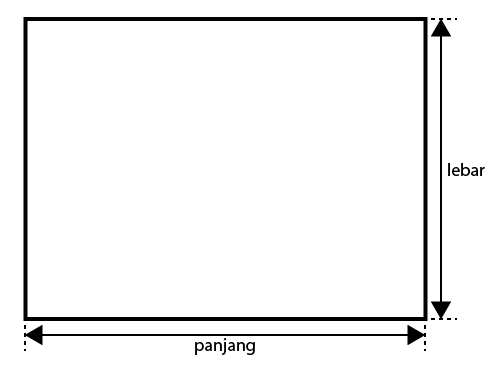
\includegraphics[scale=0.5]{model_ruangan}
	\caption[Pemodelan ruangan]{Pemodelan ruangan} 
	\label{fig:model_ruangan}
\end{figure}

%Dengan diketahuinya spesifikasi ruangan, maka akan diketahui daerah yang harus dicakup oleh kamera-kamera CCTV. Kamera-kamera CCTV akan ditempatkan dengan sedemian rupa sehingga seluruh daerah dapat tercakup. Untuk menyatakan posisi penempatan kamera CCTV, pemodelan masalah juga menggunakan sistem koordinat kertesius sehingga posisi penempatan dapat dinyatakan dalam koordinat x dan y. Dengan demikian, posisi penempatan kamera CCTV dapat dipahami lebih mudah.

\subsection{Kamera CCTV}
Hingga saat ini, sudah terdapat banyak jenis kamera CCTV yang diproduksi. Setiap kamera CCTV tersebut memiliki spesifikasinya masing-masing. Dalam permasalahan ini, terdapat 2 spesifikasi kamera CCTV yang digunakan, yaitu jarak pandang efektif dan besar sudut pandang. Gambar~\ref{fig:model_kamera} memodelkan kamera CCTV dengan kedua spesifikasi tersebut. Jarak pandang efektif adalah jarak pandang terjauh kamera CCTV untuk mengenali objek yang akan dipantau. Besar sudut pandang menunjukkan lebar pantauan kamera CCTV. Dalam permasalahan ini, jenis kamera CCTV yang digunakan hanya berjumlah 1 buah.

\begin{figure}[H]
	\centering  
	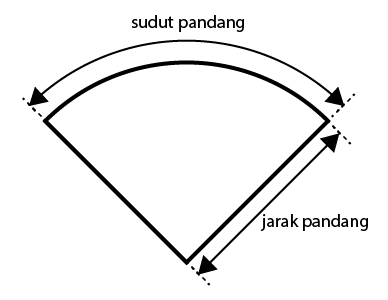
\includegraphics[scale=0.5]{model_kamera}
	\caption[Pemodelan kamera CCTV]{Pemodelan kamera CCTV} 
	\label{fig:model_kamera}
\end{figure}

\subsection{Penempatan Kamera CCTV}
Setelah ruangan dan kamera CCTV dimodelkan, selanjutnya adalah memodelkan penempatan kamera CCTV. Setiap kamera CCTV dapat ditempatkan di mana saja selama posisinya berada di dalam ruangan. Selain posisi, penempatan juga melibatkan arah pandang kamera CCTV. Posisi dan arah pandang akan mempengaruhi daerah yang dapat dicakup oleh kamera CCTV. Untuk memodelkan penempatan ini, digunakan sistem koordinat kartesius sehingga posisi penempatan dinyatakan dalam bentuk koordinat (x,y). Arah padang kamera CCTV juga dapat dinyatakan dengan besar sudut arah pandang terhadap garis \(0^\circ\) yang melewati titik posisi kamera CCTV. Posisi dan arah pandang kamera CCTV dimodelkan seperti pada gambar~\ref{fig:model_penempatan_kamera} berikut ini.

\begin{figure}[H]
	\centering  
	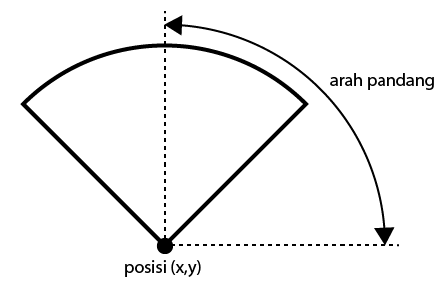
\includegraphics[scale=0.5]{model_penempatan_kamera}
	\caption[Pemodelan penempatan kamera CCTV]{Pemodelan penempatan kamera CCTV} 
	\label{fig:model_penempatan_kamera}
\end{figure}

\subsection{Daerah Cakupan}
Setiap penempatan kamera CCTV memiliki daerah yang dicakupnya masing-masing. Terdapat kasus dimana ada 2 atau lebih kamera CCTV yang mencakup suatu daerah yang sama. Daerah irisan dari cakupan-cakupan tersebut memiliki bentuk tidak sederhana sehingga sulit untuk diolah. Daerah cakupan perlu didefiniskan lebih lanjut karena menjadi bagian yang menentukan jumlah kamera CCTV. Untuk mengatasi masalah ini, daerah pada ruangan dapat dimodelkan dalam bentuk grid point seperti pada gambar~\ref{fig:model_ruangan_grid_point}. Dengan dimodelkannya ruangan dalam bentuk grid point, daerah yang harus dicakup dalam ruangan dibagi menjadi daerah-daerah yang lebih kecil atau yang disebut cell.

\begin{figure}[H]
	\centering  
	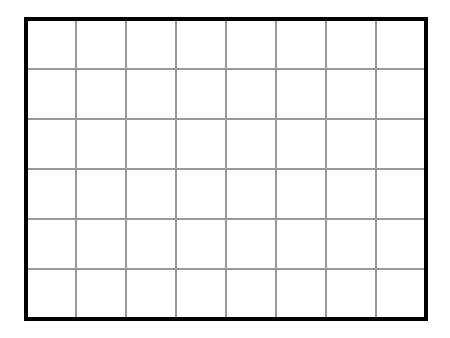
\includegraphics[scale=0.5]{model_ruangan_grid_point}
	\caption[Pemodelan ruangan dalam bentuk grid point]{Pemodelan ruangan dalam bentuk grid point} 
	\label{fig:model_ruangan_grid_point}
\end{figure}

Setiap cell dalam ruangan memiliki ukuran yang sama dengan cell-cell lainnya. Panjang harizontal dan vertikal dari cell tidak selalu berukuran sama sehingga cell dapat berbentuk persegi panjang. Penentuan ukuran cell merupakan bagian yang akan diteliti pada bagian eksperimen. Selain itu, setiap cell juga memiliki titik tengah. Titik tengah ini berfungsi sebagai titik acuan bagi kamera-kamera CCTV. Apabila titik tengah dari suatu cell berada dalam cakupan kamera CCTV, maka cell tersebut dianggap tercakup. Dengan demikian, kamera CCTV memiliki daerah cakupan yang terdiri atas kumpulan cell. Pada gambar~\ref{fig:daerah_cakupan_sebelum_grid_point} dan gambar~\ref{fig:daerah_cakupan_sesudah_grid_point}, terlihat perbedaan daerah cakupan kamera CCTV antara sebelum dan sesudah dimodelkannya ruangan dalam bentuk grid point.

\begin{figure}[H]
	\centering  
	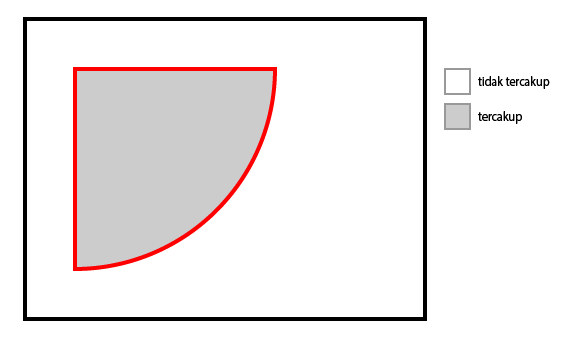
\includegraphics[scale=0.5]{daerah_cakupan_sebelum_grid_point}
	\caption[Daerah cakupan sebelum pemodelan grid point]{Daerah cakupan sebelum pemodelan grid point}
	\label{fig:daerah_cakupan_sebelum_grid_point}
\end{figure}

\begin{figure}[H]
	\centering  
	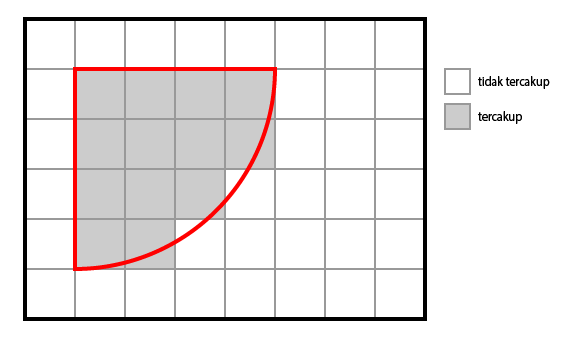
\includegraphics[scale=0.5]{daerah_cakupan_sesudah_grid_point}
	\caption[Daerah cakupan sesudah pemodelan grid point]{Daerah cakupan sesudah pemodelan grid point}
	\label{fig:daerah_cakupan_sesudah_grid_point}
\end{figure}

Cell-cell yang dicakup oleh kamera CCTV dapat dicari dengan memeriksa setiap cell pada ruangan. Pemeriksaan terdiri dari jarak cell dan sudut rotasi cell. Jarak titik tengah cell dengan posisi kamera CCTV harus lebih kecil daripada jarak pandang kamera CCTV. Sudut rotasi cell juga harus berada di antara sudut pandang kamera CCTV. Untuk mendapatkan sudut rotasi titik tengah cell terhadap posisi kamera, digunakan rumus berikut ini.
\begin{equation*}
	\theta = \tan^{-1}\left(\frac{y_2 - y_1}{x_2 - x_1}\right)
\end{equation*}
Sudut rotasi cell akan dibandingkan dengan sudut awal dan sudut akhir dari sudut pandang kamera CCTV. Apabila sudut rotasi berada di antara sudut awal dan sudut akhir, maka cell berada dalam sudut pandang kamera CCTV. Dengan memeriksa jarak dan sudut rotasi cell, cell-cell yang dicakup oleh kamera CCTV dapat ditemukan.

Dengan pemodelan grid point, tingkat overlap dan out of bound dapat dihitung dengan membandingkan jumlah cell-cell. Tingkat daerah overlap atau daerah yang dicakup oleh lebih dari 1 kamera CCTV dihitung dengan membandingkan jumlah cell overlap dengan jumlah cell pada ruangan. Sedangkan untuk menghitung tingkat daerah out of bound atau daerah cakupan yang berada di luar ruangan, dibuat cell cakupan semu yang berada di luar ruangan. Jumlah cell semu ini akan dibandingkan dengan jumlah cell di dalam ruangan sehingga didapatkan tingkat out of bound. Gambar~\ref{fig:daerah_overlap_out_of_bound} menggambarkan daerah overlap dan out of bound.

\begin{figure}[H]
	\centering  
	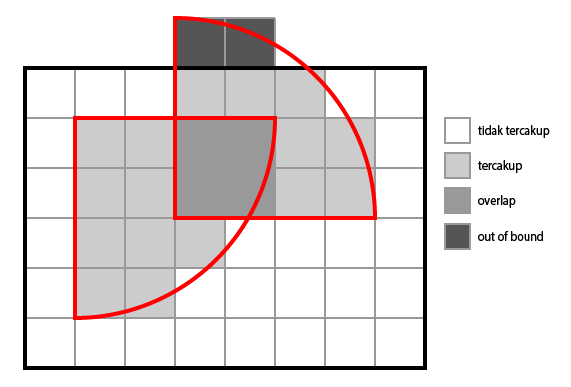
\includegraphics[scale=0.5]{daerah_overlap_out_of_bound}
	\caption[Daerah overlap dan out of bound]{Daerah overlap dan out of bound}
	\label{fig:daerah_overlap_out_of_bound}
\end{figure}

\section{Penyelesaian Masalah}
Dalam masalah ini, terdapat tujuan yang akan dicapai, yaitu mendapatkan penempatan-penempatan kamera CCTV yang dapat mencakup seluruh daerah pada ruangan dengan maksimal tingkat overlap dan out of bound sebesar 35\%. Kamera-kamera CCTV tentu dapat ditempatkan dimana saja hingga seluruh daerah pada ruangan tercakup sepenuhnya. Namun penempatan-penempatan ini tidak selalu menghasilkan tingkat overlap dan out of bound yang bernilai maksimal sebesar 35\%. Cara ini tentu tidak efektif sehingga diperlukan metode lainnya untuk menyelesaikan masalah ini. Salah satu cara yang digunakan untuk menyelesaikan masalah ini adalah dengan menggunakan linear programming.

\subsection{Variabel Keputusan}
Pada awalnya ditentukan seluruh kemungkinan penempatan kamera CCTV sehingga setiap cell pada ruangan dicakup oleh minimal 1 kamera CCTV. Setiap penempatan kamera CCTV memiliki posisi dan arah pandang masing-masing. Dari kumpulan penempatan kamera CCTV akan dicari himpunan bagian yang dimana penempatan-penempatannya dapat mencakup seluruh daerah pada ruangan dengan tingkat overlap dan out of bound yang bernilai maksimal 35\%. Setiap penempatan dalam kumpulan penempatan kamera CCTV memiliki 2 kemungkinan, yaitu diterapkan sebagai bagian dari solusi atau tidak. Dalam penyelesaian menggunakan linear programming, penempatan kamera CCTV menjadi variabel keputusan. Variabel keputusan \(x_{ij\theta}\) merujuk pada penempatan kamera CCTV pada posisi \((i,j)\) dengan arah pandang \(\theta\). Karena penempatan kamera CCTV memiliki 2 kemungkinan untuk diterapkan, maka setiap variabel keputusan dapat dinyatakan dengan nilai 0 atau 1. Apabila suatu variabel keputusan bernilai 1, maka penempatan kamera CCTV yang dirujuk akan diterapkan sebagai bagian dari solusi. Apabila benilai 0, maka penempatan kamera CCTV yang dirujuk tidak akan diterapkan. Karena variabel keputusan hanya bisa bernlai 0 dan 1 saja, masalah ini tidak diselesaikan menggunakan teknik linear programming karena hasil dapat bernilai pecahan. Masalah ini perlu diselesaikan menggunakan teknik integer programming agar hasil berbentuk bilangan bulat. Variabel keputusan dituliskan dalam bentuk berikut:
\begin{equation*}
	x_{ij\theta} =
	\left \{
  		\begin{tabular}{cl}
  			1 & jika kamera CCTV ditempatkan pada posisi $(i,j)$\\
  			  & dengan arah pandang $\theta$\\
  			  &  \\
  			0 & jika kamera CCTV tidak ditempatkan
  		\end{tabular}
  	\right.
\end{equation*}

\subsection{Fungsi Tujuan}
Solusi yang diharapkan dari masalah ini adalah penempatan-penempatan kamera CCTV yang memiliki tingkat overlap dan out of bound yang bernilai maksimal 35\%. Dengan semakin sedikitnya penempatan-penempatan kamera CCTV yang digunakan, tingkat overlap dan out of bound juga akan semakin kecil. Konsep ini sejalan dengan tujuan dari masalah. Sehingga dapat dipahami juga bahwa untuk mendapatkan tingkat overlap dan tingkat out of bound dengan maksimal 35\% juga sama dengan mencari penempatan-penempatan kamera CCTV sesedikit mungkin yang mencakup seluruh daerah pada ruangan. Sebelumnya diketahui bahwa setiap variabel keputusan hanya bisa bernilai 0 atau 1 saja. Jumlah penempatan kamera CCTV pun dapat dicari dengan menjumlahkan seluruh variabel keputusan. Fungsi tujuan dalam linear programming dapat dinyatakan sebagai jumlah penempatan kamera CCTV akan diminimalkan. Fungsi tujuan dituliskan dalam bentuk berikut:
\begin{equation*}
	\textit{minimize }z = \sum_{\theta=0}^{s_{\theta}-1} \sum_{i=0}^{s_i-1} \sum_{j=0}^{s_j-1} x_{ij\theta}
\end{equation*}

\subsection{Batasan}
Dalam menyelesaikan masalah ini, setiap daerah pada ruangan harus dicakup sepenuhnya oleh kamera-kamera CCTV.



















